\documentclass[a4paper]{article}
\usepackage[french]{babel}
\usepackage[utf8]{inputenc}
\usepackage[T1]{fontenc}
\usepackage{booktabs}   % For better-looking horizontal lines
\usepackage{array}      % For adjusting row spacing
\usepackage{csquotes}   % pour éviter un warning
\usepackage{graphicx}   % pour les images
\usepackage{hyperref}   % pour les références
\usepackage{float}      % pour les figures
% \usepackage{multicol}   % pour les 2 colonnes
\usepackage{subcaption} 
% \usepackage{caption}    % pour les légendes
% \usepackage{fullpage}   % mets les marges en petits 
% \usepackage{placeins}   % For \FloatBarrier command

\usepackage[style=ieee,backend=biber]{biblatex}
\addbibresource{ref.bib}

\hypersetup{
    colorlinks=true,
    linkcolor=blue,   % Couleur des liens internes (table des matières, références)
    citecolor=green,  % Couleur des liens vers les références bibliographiques
    filecolor=magenta,% Couleur des liens vers les fichiers
    urlcolor=blue     % Couleur des liens vers les URL
}

\title{Rapport Projet 3A \\ Analyse de trace de sang}
% \subtitle{Analyse de trace de sang}
\author{Cléa Han, Yanis Labeyrie et Adrien Zabban}
% \institute{Ecole Centrale Méditerranée, 13013 Marseille, France}
\date{Mars 2024}

\begin{document}

\maketitle

\section{Introduction}

Notre projet 3A s'intéresse à l'analyse de traces de sang dans le cadre du travail de l'expert criminalistique Philippe Esperança. En effet, l'objectif est de réaliser une intelligence artificielle pour assister et faciliter le travail d'analyse de scènes de crimes présentant du sang. 

Ce projet s'appuie sur un ensemble de données traitées et non traitées de diverses typologies de traces de sang fournies par notre expert en criminologie, ce qui nous a permis de pencher pour une solution s'appuyant sur un apprentissage supervisé. 

\section{Données}

\subsection{Données de laboratoire}
Dans un premier temps, nous avons pu manipuler des données de laboratoire, c'est-à-dire des images de traces de sang reproduites en laboratoire sur des fonds réguliers, hors des scènes de crimes. Ces fonds sont de quatre types différents : bois, lino, carrelage et papier.
Ces données de laboratoire représentent un total de 19 classes de traces de sang. Cependant, il y avait la présence d'une classe trop minoritaire parmi ces 19 classes, qui est la classe de trace d'insectes possédant uniquement quatre images. Cette classe a donc été retirée afin de garder une certaine distribution relativement équilibrée. Nous avons donc pu travailler avec 18 classes avec les données de laboratoire, pour nombre total d'images de 10 978.

La Table~\ref{tab:classes} récapitule la liste des 18 classes exploitées dans le cadre des données de laboratoire. 

\begin{table}[H]
    \centering
    \begin{tabular}{|ll|}
        \hline
        \textbf{Classe des types de trace de sang} &  \\
        \hline
        1- Modèles Traces passives & 2- Modèles Goutte à Goutte \\
        3- Modèle Transfert par contact & 4- Modèle Transfert glissé \\
        5- Modèle Altération par contact & 6- Modèle Altération glissée \\
        7- Modèle d'Accumulation & 8- Modèle Coulée \\
        9- Modèle Chute de volume & 10- Modèle sang Propulsé \\
        11- Modèle d'éjection & 12- Modèle Volume Impacté \\
        13- Modèle Imprégnation & 14- Modèle Zone d'interruption \\
        15- Modèle d'impact & 16- Modèle Foyer de modèle d'impact \\
        17- Modèle Trace gravitationnelle & 18- Modèle Sang expiré \\
        \hline
    \end{tabular}
    \caption{Liste des 18 classes utilisées des données de laboratoire}
    \label{tab:classes}
\end{table}

La Figure~\ref{fig: labs images} présentes des images de tache de sang reproduite en laboratoire. La Table~\ref{tab: images of all classes} en annexe montre un exemple de trace de sang pour chacune des 18 classes.

\begin{figure}[H]
    \centering
    \begin{subfigure}{0.40\linewidth}
        \centering
        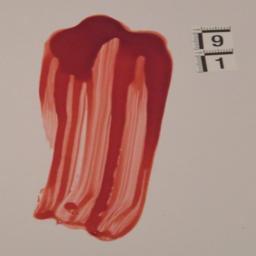
\includegraphics[width=\linewidth]{../asset/data_labo/4_papier_1586.jpg}
        \caption{Modèle Transfert glissé sur un fond de papier}
    \end{subfigure}
    \begin{subfigure}{0.40\linewidth}
        \centering
        \includegraphics[width=\linewidth]{../asset/data_labo/8_coulée_4526.jpg}
        \caption{Modèle de Coulée sur fond de lino}
    \end{subfigure}
    \caption{Deux images de laboratoire}
    \label{fig: labs images}
\end{figure}

Nous avons réparti ces données de laboratoire en 80\% dans nos données d'entraînement, 10\% dans nos données de validation et 10\% dans nos données de test. La Figure~\ref{fig:distribution labo} nous montre la distribution des données de laboratoire sur chacune des classes et chacun des datasets.

\begin{figure}[H]
    \centering
    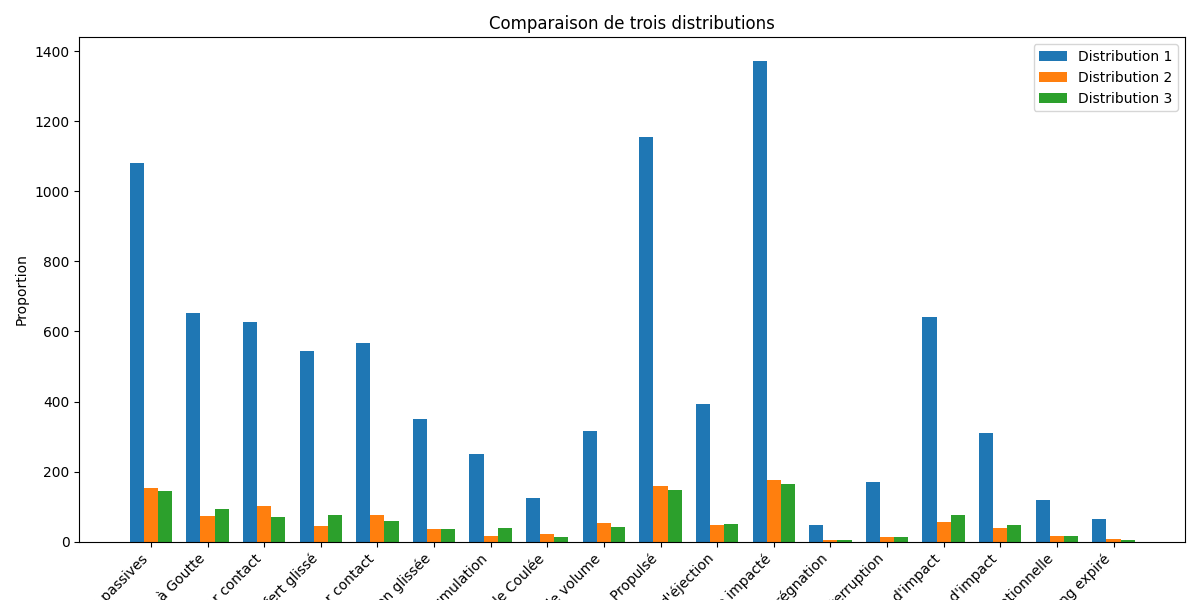
\includegraphics[width=0.8\linewidth]{../asset/distribution_train_val_test.png}
    \caption{Distribution des données de laboratoire sur les 18 classes selon le dataset d'entraînement, de validation et de teste.}
    \label{fig:distribution labo}
\end{figure}

\subsection{Données réelles issues de scène de crime}
Après l'élaboration de nos éventuels modèles pour la problématique traitée, nous avons pu manipuler des données dites réelles. Ce sont des données prises directement sur les scènes de crimes, qui sont composées de 244 images. Les images sont alors relativement moins consistantes et plus hétérogènes que les données de laboratoire. En effet, ces images sont donc issues de prises réalisées par la police scientifique, qui ne prend pas en compte les conditions consistantes de prise de photo respectées dans les données de laboratoire concoctée par Philippe Esperança. La Figure~\ref{fig: reals images} montre des exemples d'image réelles. On peut dès maintenant s'apercevoir que ces données vont être beaucoup plus compliquées à analyser pour nos modèles de deep learning au vu des nombreux objets qu'il y a sur les photos.

\begin{figure}[H]
    \centering
    \begin{subfigure}{0.40\linewidth}
        \centering
        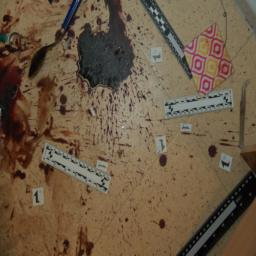
\includegraphics[width=\linewidth]{../asset/data_real/12.jpg}
        \caption{Modèle Volume Impacté}
    \end{subfigure}
    \begin{subfigure}{0.40\linewidth}
        \centering
        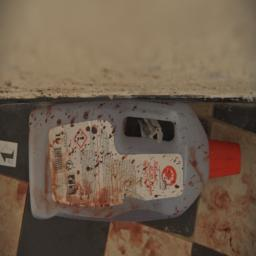
\includegraphics[width=\linewidth]{../asset/data_real/15.jpg}
        \caption{Modèle d'impact}
    \end{subfigure}
    \caption{Deux images de scène de crime}
    \label{fig: reals images}
\end{figure}

Nous avons réparti ces données réelles à 60\% dans nos données d'entraînement, à 10\% dans nos données de validation et à 30\% dans nos données de test. En effet, une plus grande proportion d'images a été attribuée au test des données réelles afin d'avoir un test relativement plus représentatif. Cet ensemble de données de test est composé de 73 images. La Figure~\ref{fig:distribution real} nous montre la distribution des données réelles sur chacune des classes et chacun des datasets.

\begin{figure}[H]
    \centering
    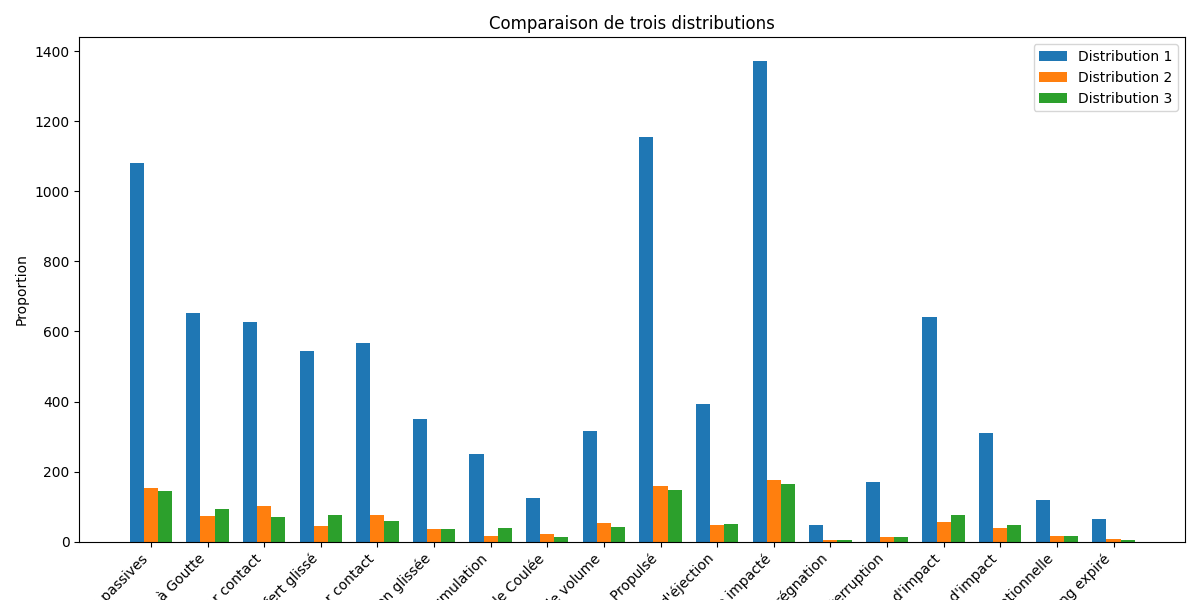
\includegraphics[width=0.8\linewidth]{../asset/distribution_train_val_test.png}
    \caption{Distribution des données de scène de crimes selon le dataset d'entraînement, de validation et de teste.}
    \label{fig:distribution real}
\end{figure}


%%%% (A voir : Idée de modèle adversarial)

\section{Modèles}

Pour aborder l'analyse de trace de sang, nous avons décidé d'utiliser le modèle Resnet pré-entraîné sur Imagenet~\cite{DBLP:journals/corr/HeZRS15} selon certains poids indiqués dans la bibliographie~\cite{torchvision2016}, selon diverses approches.

%%Afin d'adapter nos données d'entrées au mieux pour le modèle Resnet utilisé, nous avons redimensionner nos images d'entrée en taille 256 par 256. Ce qui correspond aux dimensions d'images prises en entrée par le Resnet~\cite{DBLP:journals/corr/HeZRS15}. 

Nous avons dans un premier temps retirer la dernière couche dense du modèle, qui était destiné à classifier sur 1000 catégories, puis effectuer du linear probing. Les modèles utilisant le linear probing seront désignés par LP Resnet dans la suite. Nous avons donc remplacé la dernière couche dense par 2 couches denses pour avoir une dernière couche dense à 18 neurones correspondant aux 18 classes identifiées à classifier. 

Puis, nous avons également abordé le modèle en le réentraînant sur nos données de laboratoire, c'est-à-dire effectuer du fine-tuning sur nos données. Les modèles concernés par cette méthode seront désignés par "AWL ResNet" pour All weight learnable.

Ensuite, nous avons aussi essayé d'effectuer du linear probing puis un fine-tuning de manière successive sur le modèle Resnet. Ce modèle sera désigné par le nom FT LP ResNet. 

En effet, nous avons testé plusieurs approches vis-à-vis du modèle Resnet pré-entraîné sur Imagenet afin de maximiser nos possibles performances. 

Après avoir obtenu ces différents modèles, nous les avons également fine-tuné sur l'ensemble des données réelles à notre disposition. Lorsque du fine-tuning est effectué, cela sera indiqué avec l'abréviation FT. 

%%%%% (Si ça marche : Approche adversariale)

Afin de maximiser nos potentielles performances, nous avons effectué un Grid-search afin de chercher les meilleurs hyper-paramètres possibles. 

\section{Interprétabilité}

Afin de répondre à l'aspect "boîte noire" du modèle utilisé, nous avons implémenté de l'interprétabilité dans notre modèle à l'aide de Grad-CAM~\cite{DBLP:journals/corr/SelvarajuDVCPB16}. 

Cette méthode permet de fournir une explication visuelle vis-à-vis des décisions de classification issue de notre modèle, permettant ainsi de rajouter une certaine légitimité relative face à nos analyses de traces de sang faisant partie d'un processus judiciaire. 

\section{Résultats}

Les résultats de test sur les données de laboratoire~\ref{tab:results_lab}indiquent de meilleures performances pour le modèle Resnet qui a été réentraîné sur tous ses poids, selon l'accuracy et le F1-score. 

\begin{table}[H]
  \centering
  \caption{Résultats de test sur les données de laboratoire}
    \begin{tabular}{|c|c|c|c|c|c|}
    \toprule
    Logs & Acc Micro & Acc Macro & F1-score & Top 3 \\
    \midrule
    Adversarial & 93.4\% & 91.8\% & 91.8\% & 99.8\% \\
    AWL ResNet & 97.3\% & 97.1\% & 96.2\% & 99.8\% \\
    LP ResNet & 95.2\% & 94.3\% & 94.7\% & 99.8\% \\
    \bottomrule
    \end{tabular}
  \label{tab:results_lab}
\end{table}

Les résultats de test sur les données de laboratoire~\ref{tab:results_real} indiquent de meilleures performances pour le modèle Resnet qui était entraîné entièrement sur les données de laboratoire, puis fine-tuné sur les données réelles, selon l'accuracy et le F1-score. 

\begin{table}[H]
  \centering
  \caption{Résultats de test sur les données réelles}
    \begin{tabular}{|c|c|c|c|c|c|c|}
    \toprule
    Logs & Acc Micro & Acc Macro & F1-score & Top 3 \\
    \midrule
    Adversarial & 11.8\% & 5.7\% & 3.7\% & 16.7\% \\
    FT AWL Resnet & 17.2\% & 13.8\% & 8.1\% & 28.7\% \\
    LP ResNet & 12.9\% & 6.0\% & 4.0\% & 19.0\% \\
    FT ResNet & 41.9\% & 33.4\% & 26.9\% & 51.7\% \\
    FT LP ResNet & 11.8\% & 6.1\% & 6.4\% & 26.0\% \\
    \bottomrule
    \end{tabular}
  \label{tab:results_real}
\end{table}

\section{Conclusion}

Notre projet s'inscrit dans une volonté d'optimiser le travail d'analyse de traces de sang en criminologie, notamment pour notre expert international Philippe Esperança. 

En effet, notre encadrant a pu recevoir notre projet sous la forme d'une interface qui fonctionne localement sur son appareil de travail. En effet, ce modèle d'analyse de trace de sang ne doit pas avoir accès à internet afin d'éviter tout risque d'attaque ou de fuite de données, le faire tourner en local permet de susciter la confiance de notre expert criminalistique. Il a pu apprécier et être satisfait de notre rendu.

Notre projet fait également l'objet d'une documentation afin qu'il puisse être repris aisément à l'avenir. 

\printbibliography

% \newpage
\section{Annexe}

\begin{table}[H]
    \centering
    \begin{tabular}{ccc}
        % \hline
        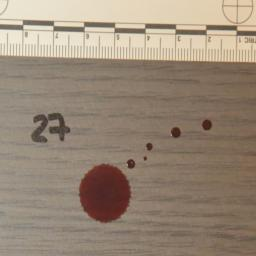
\includegraphics[width=0.25\linewidth]{../asset/data_labo/1_bois_350.jpg} & 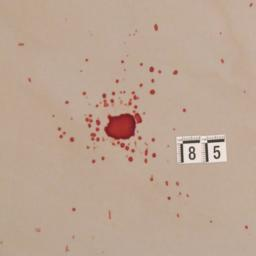
\includegraphics[width=0.25\linewidth]{../asset/data_labo/2_carrelage_523.jpg}& 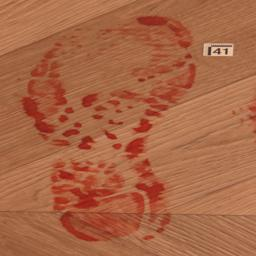
\includegraphics[width=0.25\linewidth]{../asset/data_labo/3_lino_888.jpg} \\
        1- Traces passives & 2- Goutte à Goutte & 3- Transfert par contact \\
        % \hline
        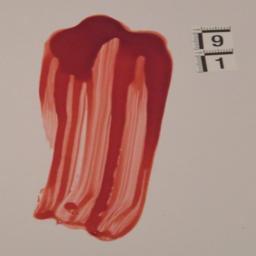
\includegraphics[width=0.25\linewidth]{../asset/data_labo/4_papier_1586.jpg} & 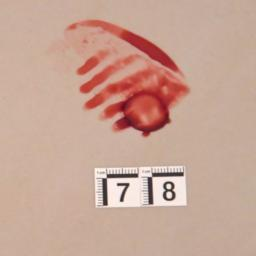
\includegraphics[width=0.25\linewidth]{../asset/data_labo/5_carrelage_5605.jpg} & 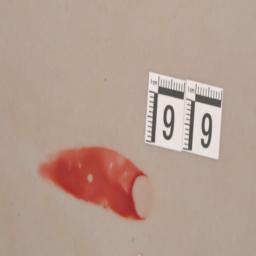
\includegraphics[width=0.25\linewidth]{../asset/data_labo/6_bois_604.jpg} \\
        4- Transfert glissé & 5- Altération par contact & 6- Altération glissée \\
        % \hline
        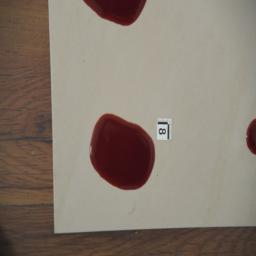
\includegraphics[width=0.25\linewidth]{../asset/data_labo/7_carrelage_5507.jpg} & \includegraphics[width=0.25\linewidth]{../asset/data_labo/8_coulée_4526.jpg} & 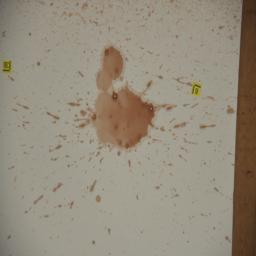
\includegraphics[width=0.25\linewidth]{../asset/data_labo/9_papier_6375.jpg} \\
        7- Accumulation & 8- Coulée & 9- Chute de volume \\
        % \hline
        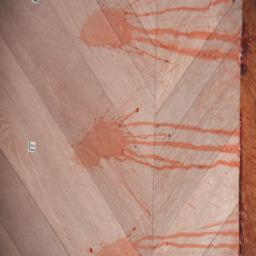
\includegraphics[width=0.25\linewidth]{../asset/data_labo/10_lino_933.jpg} & 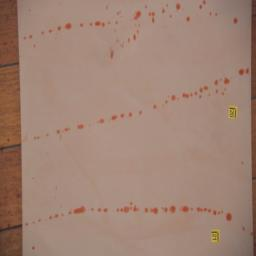
\includegraphics[width=0.25\linewidth]{../asset/data_labo/11_carrelage_905.jpg} & 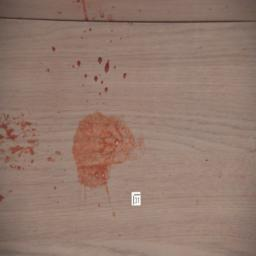
\includegraphics[width=0.25\linewidth]{../asset/data_labo/12_bois_326.jpg} \\
        10- Sang Propulsé & 11- éjection & 12- Volume impacté \\
        % \hline
        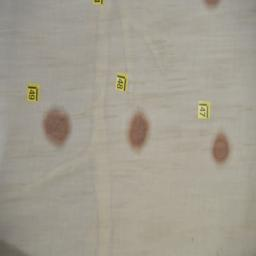
\includegraphics[width=0.25\linewidth]{../asset/data_labo/13_carrelage_7374.jpg} & 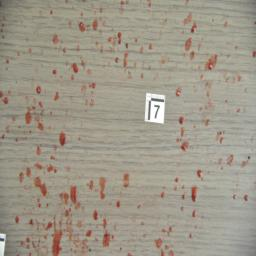
\includegraphics[width=0.25\linewidth]{../asset/data_labo/14_lino_6320.jpg} & 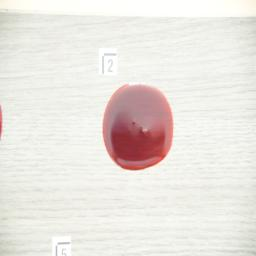
\includegraphics[width=0.25\linewidth]{../asset/data_labo/15_p1040.jpg} \\
        13- Imprégnation & 14- Zone d'interruption & 15- Modèle d'impact \\
        % \hline
        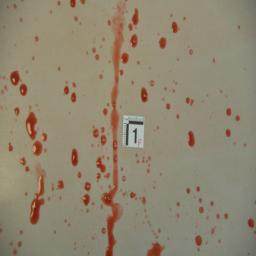
\includegraphics[width=0.25\linewidth]{../asset/data_labo/16_carrelage_598.jpg} & 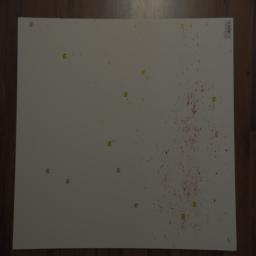
\includegraphics[width=0.25\linewidth]{../asset/data_labo/17_papier_8323.jpg} & 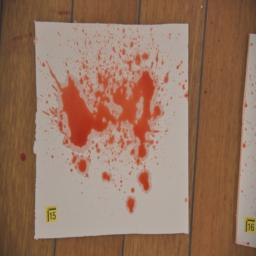
\includegraphics[width=0.25\linewidth]{../asset/data_labo/18_bois_4727.jpg}\\
        16- Foyer de modèle d'impact & 17- Trace gravitationnelle & 18- Sang expiré \\
        % \hline
    \end{tabular}
    \caption{Classe des données de laboratoire et leur exemple en image}
    \label{tab: images of all classes}
\end{table}

\end{document}
